
\documentclass{article}

\usepackage[utf8]{inputenc}
%\usepackage{fontspec}
\usepackage{xeCJK}

\usepackage{multirow}
\usepackage{hyperref}
\usepackage{float}
\usepackage{array}
\usepackage{dirtytalk}
\usepackage{csquotes}
\usepackage{amsmath}
\usepackage{graphicx}
\usepackage{amssymb}
\usepackage{pifont}

\newcommand{\cmark}{\ding{51}}%
\newcommand{\xmark}{\ding{53}}%

\title{Is Google Translate Sexist? -- Assessing Gender Bias in Machine Translation}
\author{Marcelo Prates \and Luis Lamb}

\begin{document}

\maketitle

\begin{abstract}
In recent times there has been a growing concern both inside and outside academia about the phenomenon of machine bias, where trained statistical models unbeknownst to their creators become vessels of their own prejudices. A large number of AI tools have recently been suggested to be harmfully biased towards some minority, with reports of racist criminal behavior predictors, Apple's Iphone X failing to differentiate between two Asian people and the infamous case of Google photos' classifying black people as gorillas. Although a systematic study of such biases can be difficult, we believe that automated translation tools can be exploited through gender neutral languages to yield a window into the phenomenon of \emph{gender} bias in AI. In this paper, we construct sentences with gender neutral pronouns in different languages which support them and translate these sentences into English using the Google Translate API. The resulting English sentences are constructed either with male, female or neutral pronouns, which allows us to collect statistics about the frequency of male defaults and evaluate which factors can influence the gender Google Translate assumes for each sentence. We show that not only there is a tendency towards translating pronouns to \say{he} but also that this tendency is exaggerated for sentences about male dominated fields such as computer science. At the other hand, sentences about artistic fields are less likely to yield male defaults. This possibly reflects the implicit assumptions our society has about stereotypical gender roles, which suggests that without proper care statistical machine translation can become hostage to the prejudices of those people behind its training dataset -- ourselves.
\end{abstract}

\section{Introduction}

Although the idea of automated translation can in principle be traced back to as long as the 17th century with René Descartes proposal of an \say{universal language} \cite{dascal1982universal}, machine translation has only existed as a technological field since the 1950s, with a pioneering memorandum by Warren Weaver \cite{weaver1955translation} discussing the possibility of employing digital computers to perform automated translation. The now famous Georgetown-IBM experiment followed not long after, providing the first experimental demonstration of the prospects of automating translation by the means of successfully converting more than sixty Russian sentences into English \cite{gordin2015scientific}. Early systems improved upon the results of the Georgetown-IBM experiment by exploiting Chomsky's theory of generative linguistics, and the field experienced a sense of optimism about the prospects of fully automating natural language translation. As is customary with artificial intelligence, the initial optimistic stage was followed by an extended period of strong disillusionment with the field, of which the catalyst was the influential ALPAC report \cite{hutchins1986machine}. Research was almost completely abandoned in the United States, making a shy re-entrance in the 1970s before the 1980s surge in statistical methods for machine translation \cite{koehn2009statistical}. Statistical and example-based machine translation have been on the rise ever since \cite{carl2003recent}, with highly successful applications such as Google Translate (recently ported to a neural translation technology \cite{wu2016google}) amounting to over $200$ million users daily \cite{bengio2015deep}.

In spite of the recent commercial success of automated translation tools (or perhaps stemming directly from it), machine translation has amounted a significant deal of criticism. Noted philosopher and founding father of generative linguistics Noam Chomsky has argued that the achievements of machine translation, while successes in a particular sense, are \emph{not successes in the sense that science has ever been interested in}: they merely provide effective ways, according to Chomsky, of approximating unanalyzed data. Chomsky argues that the faith of the MT community in statistical methods is absurd by analogy with a standard scientific field such as physics:

\begin{quotation}
I mean actually you could do physics this way, instead of studying things like balls rolling down frictionless planes, which can't happen in nature, if you took a ton of video tapes of what's happening outside my office window, let's say, you know, leaves flying and various things, and you did an extensive analysis of them, you would get some kind of prediction of what's likely to happen next, certainly way better than anybody in the physics department could do. Well that's a notion of success which is I think novel, I don't know of anything like it in the history of science.
\end{quotation}

Leading AI researcher and Google's Director of Research Peter Norvig responds to these arguments by suggesting that even standard physical theories such as the Newtonian model of gravitation are, in a sense, \emph{trained}:

\begin{quotation}
As another example, consider the Newtonian model of gravitational attraction, which says that the force between two objects of mass $m_1$ and $m_2$ a distance $r$ apart is given by

\begin{equation*}
F = G m_1 m_2 / r^2
\end{equation*}

where $G$ is the universal gravitational constant. This is a trained model because the gravitational constant G is determined by statistical inference over the results of a series of experiments that contain stochastic experimental error. It is also a deterministic (non-probabilistic) model because it states an exact functional relationship. I believe that Chomsky has no objection to this kind of statistical model. Rather, he seems to reserve his criticism for statistical models like Shannon's that have quadrillions of parameters, not just one or two.
\end{quotation}

Chomsky and Norvig's debate \cite{norvig2017chomsky} is a microcosmos of the two leading standpoints about the future of science in the face of increasingly sophisticated statistical models. Are we, as Chomsky seems to argue, jeopardizing science by relying on statistical tools to perform predictions instead of perfecting traditional science models, or are these tools, as Norvig argues, components of the scientific standard since its conception? Currently there are no satisfactory resolutions to this conundrum, but perhaps statistical models pose an even greater and more urgent threat to our society. On a 2014 article, Londa Schiebinger suggested that scientific research fails to take gender issues into account, arguing that the phenomenon of male defaults on new technologies such as Google Translate provides a window into this asymmetry \cite{schiebinger2014scientific}. Since then, recent worrisome results in machine learning have somewhat supported Schiebinger's view, and perhaps even partially confirmed some of Chomsky's fears. Not only Google photos' statistical image labeling algorithm has been found to classify dark-skinned people as gorillas \cite{garcia2016racist} and purportedly intelligent programs have been suggested to be negatively biased against black prisoners when predicting criminal behavior \cite{angwin2016machine} but the machine learning revolution has also indirectly revived heated debates about the controversial field of physiognomy, with proposals of AI systems capable of identifying the sexual orientation of an individual through its facial characteristics \cite{wang2017deep}. Similar concerns are growing at an unprecedented rate in the media, with reports of Apple's Iphone X face unlock feature failing to differentiate between two different Asian people \cite{womanunlockphone2017} and automatic soap dispensers which reportedly do not recognize black hands \cite{racistsoapdispenser2017}. \emph{Machine bias}, the phenomenon by which trained statistical models unbeknownst to their creators become vessels of their own prejudices, is growing into a pressing concern for the modern times, and is an invitation for us to ask ourselves whether there are limits to our dependence on these techniques -- and more importantly, whether some of these limits have already been traversed.

With this in mind, we propose a quantitative analysis of the phenomenon of gender bias in machine translation. We believe this can be done by simply exploiting Google Translate to map sentences from a gender neutral language to English. As Figure \ref{fig:screenshot-gtranslate-hungarian} exemplifies, this approach produces results consistent with the hypothesis that senteces about stereotypical gender roles are translated accordingly with high probability: \emph{nurse} and \emph{baker} are translated with female pronouns while \emph{engineer} and \emph{CEO} are translated with male ones.

\begin{figure}[h]
	\centering
	\fbox{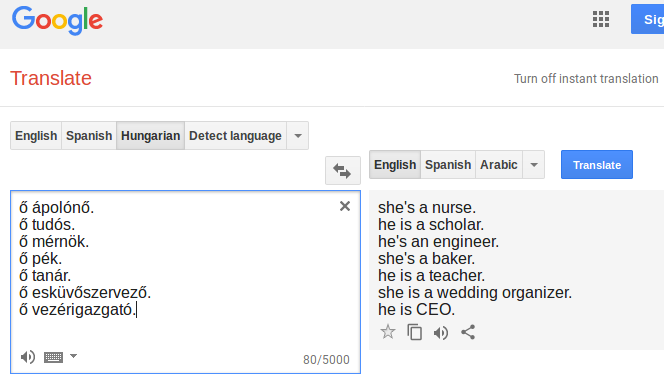
\includegraphics[width=\linewidth]{pictures/screenshot-gtranslate-hungarian}}
	\label{fig:screenshot-gtranslate-hungarian}
	\caption{Translating sentences from a gender neutral language such as Hungarian to English provides a glimpse into the phenomenon of gender bias in machine translation. This screenshot from Google Translate shows how occupations from traditionally male-dominated fields such as scholar, engineer and CEO are interpreted as male, while occupations such as nurse, baker and wedding organizer are interpreted as female.}
\end{figure}

\section{Motivation}

If automatic translation tools are indeed gender biased as Figure \ref{fig:screenshot-gtranslate-hungarian} seems to suggest, then possibly this phenomenon can be probed to yield many valuable insights. One could in principle group different professional occupations according to their broad category (artistic, scientific, industrial, etc.) and evaluate whether the proportion of male pronouns is more pronounced in some fields compared to others. We expect, for example, that most sentences about computer-related jobs will be translated with male pronouns, as a reflection of the gender asymmetry of this job market. We can also collect translation statistics among varied gender neutral languages to see whether different cultures make different assumptions about the gender of a subject.

If conclusive, in our view such an analysis would suggest that automatic translation tools should be designed in such a way as to avoid becoming hostages to their own underlying statistical models. Because these tools are trained with real world data they implicitly absorb the biases and stereotypes of our society, which must then be painstakingly removed. This poses an ethical rather than a technical limitation to statistical machine translation and big data statistical models in general.

\section{Methods}

We believe that the phenomenon of gender bias in machine translation can be assessed by mapping sentences constructed in gender neutral languages to English by the means of an automated translation tool. Specifically, we can translate sentences such as the Hungarian \say{ő ápolónő}, where \say{ápolónő} translates to \say{nurse} and \say{ő} is a gender-neutral pronoun meaning either he, she or it, to English, yielding in this example the result \say{she's a nurse} on Google Translate. The same basic template can be ported to all other gender neutral languages, as Table \ref{tab:templates} shows. Given the success of Google Translate, which amounts to 200 million users daily, we have decided to exploit its API to obtain the desired thermometer of gender bias. Also, in order to solidify our results, we have decided to work with as many gender neutral languages as possible, obtaining a list of these from the Wikipedia article on the issue (\url{https://en.wikipedia.org/wiki/Gender_neutrality_in_genderless_languages}). Table \ref{tab:gender-neutral-languages} compiles all languages from said article, with additional columns informing whether they 1) exhibit a pronominal gender system and 2) are supported by Google Translate. Because pronominal gender systems defy the purposes of our technique, such languages have been discarded. Following difficulties with Bengali, Nepali and Korean we have decided not to work with these languages also.

There is a prohibitively large class of nouns and adjectives that could in principle be substituted in the templates of Table \ref{tab:templates}. To simplify our dataset, we have decided to obtain a comprehensive list of professional occupations, which, we believe, are an interesting window into the nature of gender bias. Once again we resorted to a Wikipedia article (\url{https://en.wikipedia.org/wiki/Lists_of_occupations}) to collect this data, of which the statistics of occupations per category (Artistic, Corporate, Theatre, etc.) are shown in Table \ref{tab:occupations}. Finally, Table \ref{tab:occupations-examples} shows thirty examples of randomly selected occupations from our dataset. Finally, we have selected a small list of 21 adjectives, presented in Table \ref{tab:adjectives}.

\begin{table}[H]
	\centering
	\begin{tabular}{|c|m{2cm}|m{2cm}|c|c|}
	\hline
	Language Family & Language & Pronominal Gender System & Supported & Tested \\ \hline \hline
	\multirow{2}{*}{Austronesian} 	& Malay 				& \xmark 			& \checkmark	& \checkmark	\\
									& Tagalog 				& \xmark 			& \xmark		& \xmark		\\ \hline
	\multirow{3}{*}{Finno-Ugric} 	& Estonian 				& \xmark 			& \checkmark 	& \checkmark	\\
									& Finnish 				& \xmark 			& \checkmark	& \checkmark	\\
									& Hungarian 			& \xmark 			& \checkmark 	& \checkmark	\\ \hline
	\multirow{4}{*}{Indo-European} 	& Armenian 				& \xmark 			& \checkmark 	& \checkmark	\\
									& Bengali 				& \xmark 			& \checkmark 	& \xmark		\\
									& English 				& \checkmark 		& \checkmark 	& \xmark 		\\
									& Persian 				& \checkmark 		& \checkmark 	& \xmark 		\\ \hline
	\multirow{3}{*}{Indo-Aryan} 	& Maithili 				& \xmark 			& \xmark 		& \xmark 		\\
									& Nepali 				& \xmark 			& \checkmark	& \xmark		\\
									& Oriya 				& \xmark 			& \xmark 		& \xmark 		\\ \hline
	\multirow{10}{*}{} 				& Japanese 				& \xmark 			& \checkmark 	& \checkmark	\\
									& Korean 				& O 				& \checkmark 	& \xmark		\\
									& Turkish 				& \xmark 			& \checkmark 	& \checkmark	\\
									& Yoruba 				& \xmark 			& \checkmark 	& \checkmark	\\
									& Basque 				& \xmark 			& \checkmark 	& \checkmark	\\
									& Swahili 				& \xmark 			& \checkmark 	& \checkmark	\\
									& Chinese 				& O 				& \checkmark 	& \checkmark	\\
									& Cantonese 			& \xmark 			& \xmark		& \xmark		\\
									& Pipil 				& \xmark 			& \xmark		& \xmark		\\
									& Quechuan 				& \xmark 			& \xmark		& \xmark		\\ \hline
	\multirow{4}{*}{Constructed} 	& Esperanto 			& \checkmark 		& \checkmark 	& \xmark		\\
									& Ido 					& O 				& \xmark 		& \xmark 		\\
									\cline{2-2}
									& Lingua Franca Nova 	& \xmark 			& \xmark 		& \xmark 		\\
									\cline{2-2}
									& Interlingua 			& \xmark 			& \xmark 		& \xmark 		\\ \hline
	\end{tabular}
	\caption{Selected gender neutral languages obtained from the Wikipedia article \url{https://en.wikipedia.org/wiki/Gender_neutrality_in_genderless_languages}. Languages are grouped according to language families and classified according to whether they exhibit pronominal gender system (\checkmark: yes, \xmark:~no, O: it is optional). For the purposes of this work, we have decided to work only with languages lacking such a system, and as such Persian and Esperanto have been discarded. Languages lacking support from Google Translate have been discarded. Following difficulties with Bengali, Nepali and Korean, these languages have also been discarded.}
	\label{tab:gender-neutral-languages}
\end{table}

\begin{table}[H]
	\centering
	\begin{tabular}{|c|c|}
	\hline
	Category 		& \# Occupations 	\\ \hline \hline
	Artistic 		& $102$ 			\\ \hline
	Computer 		& $19$ 				\\ \hline
	Corporate 		& $50$ 				\\ \hline
	Dance 			& $9$ 				\\ \hline
	Film/Television & $26$ 				\\ \hline
	Healthcare 		& $88$ 				\\ \hline
	Industrial 		& $26$ 				\\ \hline
	Science 		& $50$ 				\\ \hline
	Service 		& $10$ 				\\ \hline
	Theatre 		& $52$ 				\\ \hline
	Writing 		& $29$ 				\\ \hline
	\hline
	Total			& $462$				\\ \hline
	\end{tabular}
	\caption{Selected occupations obtained from the Wikipedia article \url{https://en.wikipedia.org/wiki/Lists_of_occupations}, grouped by category. We have selected a total of 462 occupations from $11$ distinct groups (Artistic, Science, Service, etc.).}
	\label{tab:occupations}
\end{table}

\begin{table}[H]
	\centering
	\begin{tabular}{|c|c|}
	\hline
	Language 	& Sentence template \\ \hline \hline
	Malay		& dia adalah $\langle occupation \rangle$ \\ \hline
	Estonian	& ta on $\langle occupation \rangle$ \\ \hline
	Finnish		& hän on $\langle occupation \rangle$ \\ \hline
	Hungarian	& ő $\langle occupation \rangle$ \\ \hline
	Armenian	& նա $\langle occupation \rangle$ է \\ \hline
	Japanese	& $\langle occupation \rangle$ です\\ \hline
	Turkish		& o bir $\langle occupation \rangle$ \\ \hline
	Yoruba		& o jẹ $\langle occupation \rangle$ \\ \hline
	Basque		& $\langle occupation \rangle$ da \\ \hline
	Swahili		& yeye ni $\langle occupation \rangle$ \\ \hline
	Chinese		& ta $\langle occupation \rangle$ \\ \hline
	\end{tabular}
	\caption{Templates used to infer gender biases in the translation to the English language.}
	\label{tab:templates}
\end{table}

\begin{table}[H]
	\centering
	\begin{tabular}{|c|c|c|c|c|}
	\hline
	stagehands & author & neurologist \\ \hline
	screenwriter & animator & marketing director \\ \hline
	biochemist & endocrinologist & freelancer \\ \hline
	neurosurgeon & computer scientist & petrochemical engineer \\ \hline
	food stylist & cardiothoracic surgeon & property master \\ \hline
	literary editor & video editor & animation director \\ \hline
	house manager & chief administrative officer & arts administration \\ \hline
	actor & dialysis technician & family nurse practitioner \\ \hline
	psychologist & chief creative officer & flash developer \\ \hline
	scenic artist & producer & medical laboratory scientist \\ \hline
	\end{tabular}
	\caption{A randomly selected example subset of thirty occupations obtained from our dataset with a total of 462 different occupations.}
	\label{tab:occupations-examples}
\end{table}

\begin{table}[H]
	\centering
	\begin{tabular}{|c|c|c|}
	\hline
	happy 		& sad 		& right 	\\ \hline
	wrong 		& afraid	& brave 	\\ \hline
	smart		& dumb		& proud 	\\ \hline
	ashamed		& kind		& cruel 	\\ \hline
	envious		& loving	& hateful 	\\ \hline
	modest 		& arrogant	& guilty	\\ \hline
	innocent	& helpless	& shy		\\ \hline
	\end{tabular}
	\caption{Adjectives}
	\label{tab:adjectives}
\end{table}

\section{Results}

For each one of the tested 462 occupations (see Tables \ref{tab:occupations}, \ref{tab:occupations-examples}), we used the Python Google Translate API (\url{http://py-googletrans.readthedocs.io/en/latest/}) to translate sentences built with the templates in Table \ref{tab:templates} from each one of the tested languages in Table \ref{tab:gender-neutral-languages} to English. The resulting sentences are then classified as \emph{female}, \emph{male} or \emph{neutral} according to their respective pronouns. Sentences starting with \say{She/She's/Her} are classified as female, sentences starting with \say{He/He's/His} are classified as male and sentences starting with \say{It/It's/Its/They/They're/Their} are classified as (gender) neutral. The results from this analysis, which can be found in \url{https://github.com/marceloprates/Gender-Bias}, are further discussed below.

One can see either in Table \ref{tab:gender-by-category} or Figure \ref{fig:gender-by-category} that not only does Google Translate exhibit a tendency towards male defaults, but also that this tendency is further enhanced for typically male dominated fields such as computer science (with a ratio of $17.857$ male pronouns per female pronoun). Sentences about occupations from the \emph{Corporate} and \emph{Science} category are also disproportionately translated with male pronouns (sex ratios $9.444$ and $10.5$ respectively), while those containing occupations from the \emph{Dance} category achieve a sex ratio of almost one ($1.064$). Not one category has achieved a balanced sex ratio, neither does any category exhibit more gender neutral than male pronouns. In total, female pronouns add up to $16.522\%$ among all categories, while male pronouns add up to $63.083\%$ and gender neutral pronouns to just $7.912\%$, yielding an average sex ratio of $3.818$.

\begin{table}[H]
	\centering
	\begin{tabular}{|c|c|c|c|c|c|}
	\hline
	Category & Female & Male & Neutral & Ratio & Total \\ \hline
	\hline
	Artistic        & 188 & 518 & 72 & 2.755 	& 918 \\ \hline
	Computer        & 7   & 125 & 12 & 17.857 	& 171 \\ \hline
	Corporate       & 36  & 340 & 23 & 9.444 	& 450 \\ \hline
	Dance           & 31  & 33  & 8  & 1.064 	& 81  \\ \hline
	Film-television & 54  & 125 & 18 & 2.315 	& 234 \\ \hline
	Healthcare      & 176 & 483 & 64 & 2.744 	& 792 \\ \hline
	Industrial      & 40  & 135 & 29 & 3.375   	& 234 \\ \hline
	Science         & 34  & 357 & 25 & 10.500	& 450 \\ \hline
	Service         & 5   & 63  & 10 & 12.600	& 90  \\ \hline
	Theatre         & 75  & 296 & 38 & 3.947 	& 477 \\ \hline
	Writing         & 41  & 148 & 30 & 3.610 	& 261 \\ \hline
	\hline
	Total           & 687 & 2623 & 329 & 3.818 & 4158 \\ \hline
	\end{tabular}
	\label{tab:gender-by-category}
	\caption{Number of female, male and neutral pronominal genders per occupation category in the translated sentences. The corresponding sex ratios (\# Male / \# Female) show just how much male defaults are prominent in male dominated fields such as computer science, with up to $\approx 18$ occurrences of male pronouns for each of a female one.}
\end{table}

\begin{figure}[H]
	\centering
	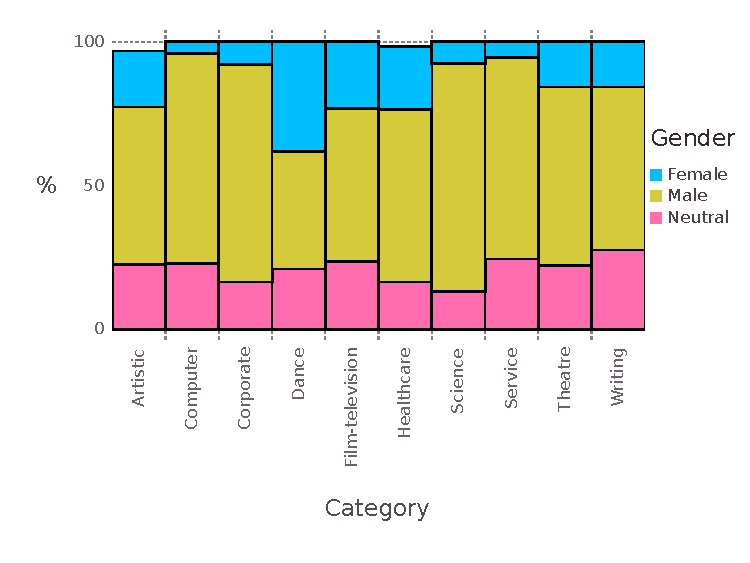
\includegraphics[width=\linewidth]{pictures/gender-by-category}
	\label{fig:gender-by-category}
	\caption{The distribution of pronominal genders in the translated sentences not only suggests a tendency towards male defaults but also reflects the structure of male dominated fields, with the proportion of male pronouns amounting to $73\%$ in computer related jobs and $76\%$ in corporate jobs respectively. Because Google Translate occasionally fails to translate a sentence, the bars for some categories fail to add up to $100\%$.}
\end{figure}

While grouping translations by category helps shed light on the stereotypical gender roles among different professions, grouping translations by language can help us understand the effect each culture possibly has on this issue. Table \ref{tab:gender-by-language} shows some sex ratios even larger than the previous ones, particularly when translating from Yoruba ($25.333$), Chinese ($27.5$) and Japanese, the last one peaking at an impressive ratio of $107.5$ male per female pronouns. Figure \ref{fig:gender-by-language} shows that, when grouping by language, gender neutral pronouns can be more prominent than male pronouns at least in one case: translating sentences from Basque yields 153 neutral vs 50 male and 5 female pronouns. Unfortunately this is the exception rather than the rule, with Yoruba following after with 131 neutral vs 304 male and 12 female pronouns. In total, female pronouns add up to $18.687\%$ among all categories, while male pronouns add up to $81.626\%$ and gender neutral pronouns to $8.466\%$, yielding an average sex ratio of $4.368$ ($14.405\%$ larger than what we get from grouping among categories). It should be noted however that Japanese and Basque, the two languages which stood out from the behavior observed in Figure \ref{fig:gender-by-category}, are precisely the two that Google Translate found hardest to translate. These findings should, as a result, be taken with a grain of salt.

\begin{table}[H]
	\centering
	\begin{tabular}{|c|c|c|c|c|c|}
	\hline
	Language & Female & Male & Neutral & Ratio & Total \\ \hline
	\hline
	Malay     & 47  & 415  & 0   & 8.830 	& 462 \\ \hline
	Estonian  & 130 & 332  & 0   & 2.554 	& 462 \\ \hline
	Finnish   & 179 & 283  & 0   & 1.581 	& 462 \\ \hline
	Hungarian & 189 & 270  & 1   & 1.429 	& 462 \\ \hline
	Armenian  & 101 & 360  & 1   & 3.564 	& 462 \\ \hline
	Japanese  & 2   & 215  & 0   & 107.500  & 462 \\ \hline
	Turkish   & 22  & 394  & 43  & 17.909	& 462 \\ \hline
	Yoruba    & 12  & 304  & 131 & 25.333	& 462 \\ \hline
	Basque    & 5   & 50   & 153 & 10.000   & 462 \\ \hline
	Swahili   & 76  & 386  & 0   & 5.079 	& 462 \\ \hline
	Chinese   & 14  & 385  & 23  & 27.500   & 462 \\ \hline
	\hline
	Total     & 777 & 3394 & 352 & 4.368	& 4158   \\ \hline
	\end{tabular}
	\caption{Number of female, male and neutral pronominal genders per language in the translated sentences. The corresponding sex ratios (\# Male / \# Female) show just how much male defaults are prominent in some languages such as Chinese, with almost 30 male pronouns for each female one.}
	\label{tab:gender-by-language}
\end{table}

\begin{figure}[H]
	\centering
	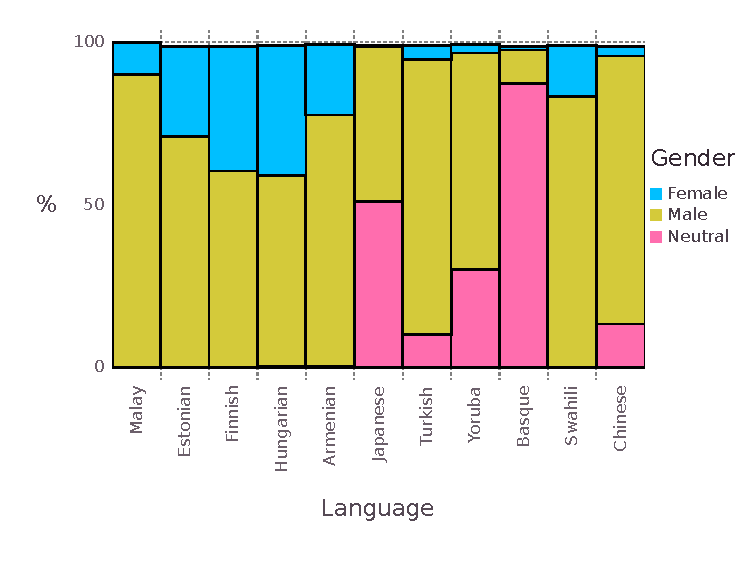
\includegraphics[width=\linewidth]{pictures/gender-by-language}
	\label{fig:gender-by-language}
	\caption{The distribution of pronominal genders per language also suggests a tendency towards male defaults, with female pronouns reaching as low as $0.46\%$ and $2.98\%$ for Japanese and Chinese respectively. Once again not all bars add up to $100\%$ as Google Translate occasionally fails to translate sentences, particularly in Japanese and Basque. Among all tested languages, Basque was the only one to yield more gender neutral than male pronouns.}
\end{figure}

Instead of grouping sentences either by category or language, we can also visualize each of them individually on a scatter plot. Figure \ref{fig:scatterplot-languages} shows each occupation as a point on a bi-dimensional lattice, arranged horizontally by their sex ratio and vertically by the proportion of gender neutral pronouns, both averaged over translations from all tested languages. Each point is also color coded according to that occupation's respective category (Artistic, Writing, Science, etc.).

\begin{figure}[H]
	\centering
	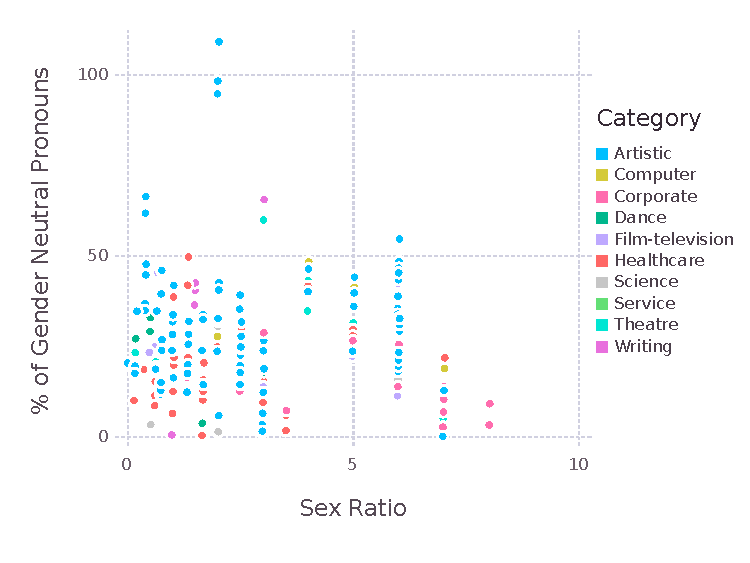
\includegraphics[width=\linewidth]{pictures/scatterplot-languages}
	\label{fig:scatterplot-languages}
	\caption{Scatter plot of translated sentences' statistics. Each point (color coded according to its category) corresponds to a single occupation, of which the sex ratio and the percentage of gender neutral pronouns are averaged over all tested languages (Malay, Estonian, Finnish, Hungarian, Armenian, Japanese, Turkish, Yoruba, Basque, Swahili and Chinese).}
\end{figure}

Figures \ref{fig:histogram-female}, \ref{fig:histogram-female} and \ref{fig:histogram-neutral} shed further light on the asymmetry between the distribution male and female pronouns. While the number of occurences of male pronouns tends towards a normal distribution, the figure is changes drastically for the opposite gender, whose pronoun distribution is apparently governed by an inverse correlation. The behavior repeats itself for the gender neutral pronouns in Figure \ref{fig:histogram-neutral}.

\begin{figure}[H]
	\centering
	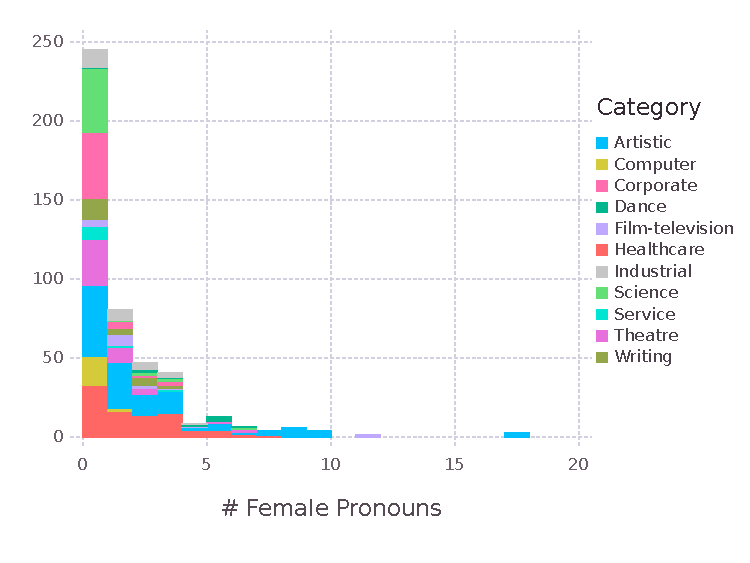
\includegraphics[width=\linewidth]{pictures/histogram-female}
	\caption{Histogram of the distribution of female pronouns among different occupation categories, with a distinctive peak at 0. The corresponding histogram for male pronouns (see Figure \ref{fig:histogram-male}), by constrast, peaks at 9.}
	\label{fig:histogram-female}
\end{figure}

\begin{figure}[H]
	\centering
	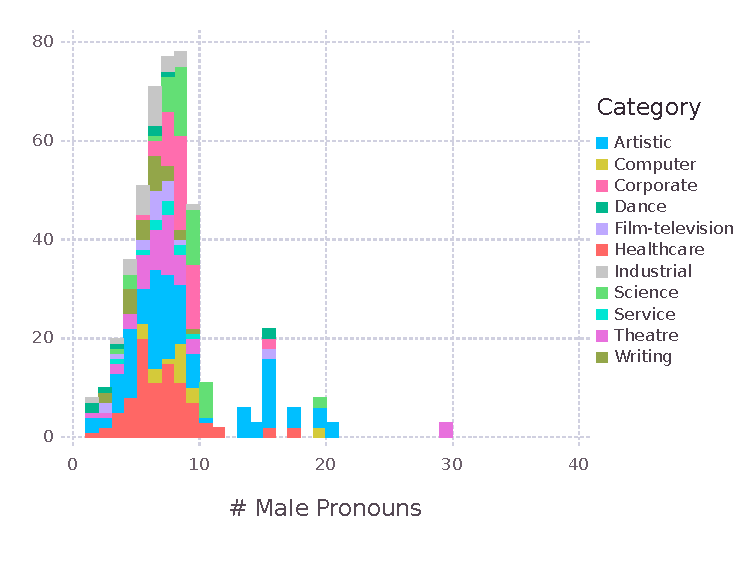
\includegraphics[width=\linewidth]{pictures/histogram-male}
	\caption{Histogram of the distribution of male pronouns among different occupation categories, with a distinctive peak at 9. In contrast with the corresponding histograms for female and gender neutral pronouns (see Figures \ref{fig:histogram-female} and \ref{fig:histogram-neutral} respectively) which exhibit inverse correlations, here one can see a tendency towards normally-distributed pronoun counts.}
	\label{fig:histogram-male}
\end{figure}

\begin{figure}[H]
	\centering
	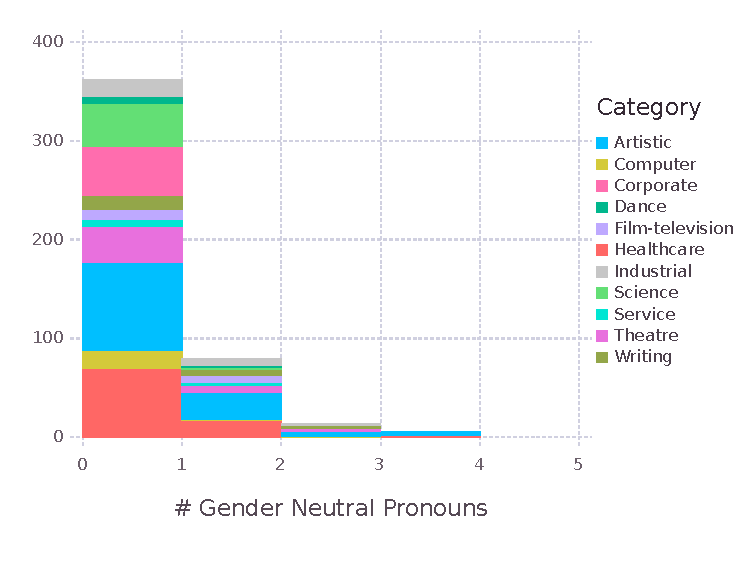
\includegraphics[width=\linewidth]{pictures/histogram-neutral}
	\caption{Following the behavior observed for female pronouns, the histogram for the distribution of gender neutral pronouns among different categories shows a tendency towards an inverse correlation, with a distinctive peak at 0.}
	\label{fig:histogram-neutral}
\end{figure}

Finally, Figure \ref{fig:barplot-adjectives} and Table \ref{tab:gender-by-adjective} show how stereotypical gender roles possibly play a part when simple adjectives are translated. We observed that objective statements such as \say{he/she is wrong/right/guilty/innocent} are biased towards male defaults, while statements concerning emotional states (\say{sad},\say{kind},\say{shy}) amass at the opposite extreme of the sex ratio spectrum. Unsurprisingly, the statement \say{he/she is attractive} is translated predominately with female pronouns.

\begin{table}[H]
	\centering
	\begin{tabular}{|c|c|c|c|c|c|}
	\hline
	Adjective 	& Female & Male & Neutral & Ratio & Total \\ \hline
	\hline
	Shy     	& 6  & 2   & 2  & 0.333 	& 12  \\ \hline
	Attractive 	& 4  & 2   & 4  & 0.500   	& 12  \\ \hline
	Happy   	& 5  & 3   & 2  & 0.600   	& 12  \\ \hline
	Kind    	& 4  & 3   & 1  & 0.750 	& 12  \\ \hline
	Ashamed 	& 4  & 5   & 1  & 1.250 	& 12  \\ \hline
	Smart   	& 2  & 5   & 3  & 2.500   	& 12  \\ \hline
	Envious 	& 2  & 6   & 1  & 3.000   	& 12  \\ \hline
	Sad     	& 2  & 6   & 2  & 3.000   	& 12  \\ \hline
	Loving  	& 2  & 6   & 2  & 3.000   	& 12  \\ \hline
	Helpless 	& 2  & 6   & 2  & 3.000   	& 12  \\ \hline
	Brave   	& 2  & 7   & 1  & 3.500   	& 12  \\ \hline
	Proud   	& 2  & 7   & 1  & 3.500   	& 12  \\ \hline
	Hateful 	& 1  & 5   & 3  & 5.000   	& 12  \\ \hline
	Dumb    	& 1  & 6   & 2  & 6.000   	& 12  \\ \hline
	Innocent 	& 1  & 8   & 1  & 8.000   	& 12  \\ \hline
	Right   	& 0  & 7   & 3  & -   		& 12  \\ \hline
	\hline
	Total   	& 43 & 129 & 41 & 3     	& 264 \\ \hline
	\end{tabular}
	\caption{Number of female, male and neutral pronominal genders in the translated sentences for each selected adjective.}
	\label{tab:gender-by-adjective}
\end{table}

\begin{figure}[H]
	\centering
	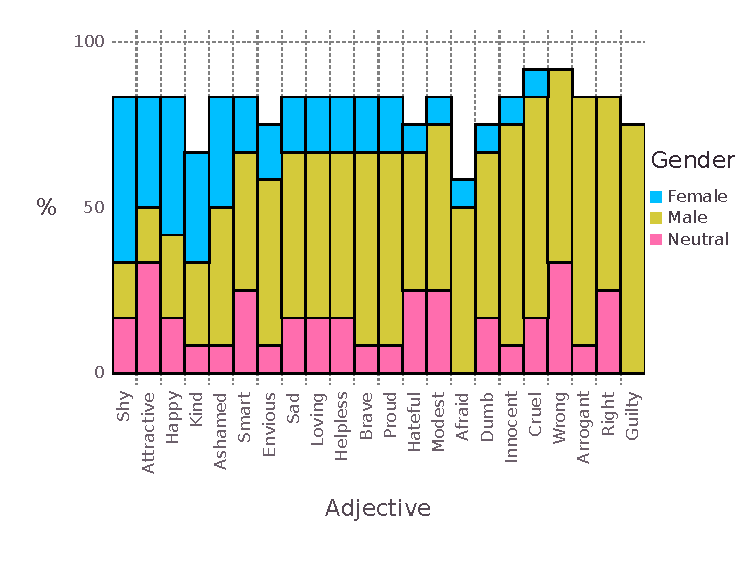
\includegraphics[width=\linewidth]{pictures/barplot-adjectives}
	\caption{The distribution of pronominal genders for each word in Table \ref{tab:adjectives} shows how stereotypical gender roles can play a part on the automatic translation of simple adjectives. One can see that adjectives such as \emph{shy} and \emph{attractive} are predominantly translated with female pronouns, while words like \emph{guilty}, \emph{innocent}, \emph{wrong}, \emph{right}, \emph{arrogant} are almost exclusively translated with male pronouns. Objective statements have a tendency towards male defaults, while statements concerning emotional states (\emph{shy}, \emph{happy}, \emph{kind}, \emph{ashamed}) amass at the other extreme of the sex ratio spectrum.}
	\label{fig:barplot-adjectives}
\end{figure}

\section{Discussion}

In this paper, we have provided evidence that statistical translation tools such as Google Translate exhibit implicit gender biases and a tendency towards male defaults, which possibly stem from the real world data used to train them. As a result, we suggest that such tools can be probed to yield insights about stereotypical gender roles in our society. By translating sentences from gender neutral languages such as Hungarian and Chinese into English, we were able to collect statistics about the asymmetry between female and male pronominal genders in the translation process. Because Google Translate typically uses English as a \emph{lingua franca} to translate between other languages, our findings probably generalize to most translations from gender neutral idioms, although we have not tested this hypothesis. Our results further show that although male pronouns are typical, the proportion of female pronouns can vary significantly according either to the adjectives used (\say{shy}/\say{happy} vs \say{brave}/\say{Guilty}) or the category of professional occupations (artistic jobs are far more likely to be translated with female pronouns than computer-related ones). We have also shown that different languages are differently biased towards male defaults, with Hungarian exhibiting a better balance between male and female pronouns than, say, Chinese. Some languages such as Yoruba and Basque have been found to translate sentences with gender neutral pronouns very often, although this is the exception rather than the rule.

We think this work can shed further light on some of the technical and ethical difficulties that arise from statistical machine translation, and hope that it arouses discussions about the role of AI engineers on minimizing the harmful effects of the pressing modern concern of machine bias.

\clearpage
\bibliographystyle{unsrt}
\bibliography{main}

\end{document}